\section{Definition von SIEMs und Log-Analyse-Tools}

Sowohl in der wissenschaftlichen als auch in der kommerziellen Literatur gibt es verschiedene Definitionen von \gls{SIEM}. Diese widersprechen sich nicht, aber zeigen unterschiedliche Perspektiven. Eine von dieser Definitionen behaupt, dass \gls{SIEM} das Ergebnis einer Kombination zwischen dem \glsfirst{SEM} und \glsfirst{SIM} ist \citep{Dorigo_SIEM}. Das Erste bezieht sich auf die Identifizierung, Bewertung, Beobachtung und den Bericht von Sicherheitsvorfällen mithilfe von verschiedenen Log Dateien \citep{techopedia_SEM}. Das Zweite ist eine Software, die bei der automatischen Sammlung von Loginformationen aus vielen Quellen, wie Firewall und Servern unterstützt \citep{techopedia_SIM}. Da die meisten \gls{SIEM}-Lösungen kostenpflichtig sind, existieren auch viele \gls{opensource} Log-Analyse-Tools, die eine ähnliche Aufgabe erledigen, ohne die Kernelemente von \gls{SIEM} zu besitzen.

Log-Analyse-Tools sind in der Regel Anwendungen die Logdateien empfangen, speichern, bearbeiten und nach spezifisichen Regeln bewerten. Diese Tools unterstützen Programmierer und Systemadministratoren bei der Überwachung des Zustands von Systems oder einer Software. Ein solches Tools kann Logdateien von verschiedenen \glsplural{Endpoint} und in verschiedenen Formaten bekommen, so dass es schließlich einen Bericht oder eine Grafik erzeugt \citep{Korzeniowski_LATDef}. Ihre Nutzung beschränkt sich nicht auf den Sicherheitsbereich ein, sondern kann für gesamte IT-Bereich nützlich sein.

In dem Universum des \gls{SOC} mischen sich verschiedene Begriffe, die manchmal zur Verwirrung führen, weil sie ähnliche Bedeutungen haben und Verantwortungen abdecken. \glsfirst{IDS}, \glsfirst{IPS}, \glsfirst{SIEM} und Log-Analyse-Tools werden von Laien und sogar von Spezialisten oft verwechselt, da ihre Aufgaben mehr Gemeinsamkeiten als Unterschiede haben. Diese Tools sind feste Bestandteil eines \gls{SOC}, jedoch konzentrieren wir uns auf Log-Analyse. Um den Fokus der Arbeit zu vergrenzen, erläutern wir demnächst Abschnitt die erwähnten Begriffe.

\glsfirst{IDS}, \glsfirst{IPS} und \glsfirst{SIEM} sind Sicherheitstool als Software und/oder Hardware, die zusammenarbeiten können, um einen umfangreiche Netzwerksicherheit anzubieten. \gls{IDS} identifizieren und berichten über \glsplural{Cyberangriff}, indem er Netzwerkverkehr überwacht. Nach der Erkennung eines verdächtigen Verkehrs, muss das \gls{SOC} Team zur Handlung kommen. \gls{IPS} überwacht den Netzwerkverkehr und kann die Verbindung automatisch unterbrechen, falls es verdächtig ist \citep{Wendzel_IS}. Ein \gls{IPS} kann konfiguriert werden, um automatisch nach festgelegten Muster zu handeln. Beide Tools können Logdateien generieren, die von einer \gls{SIEM}-Lösung oder Log-Analyse-Tools gesammelt werden können. Die Abbildung \ref{fig:SIEM_Allg_Struktur} stellt eine allgemeine Struktur von \gls{SIEM}-Lösungen dar:

%\textbf{\textcolor{red}{Graphik selbst bauen}}

\begin{figure}[H]
   \centering
   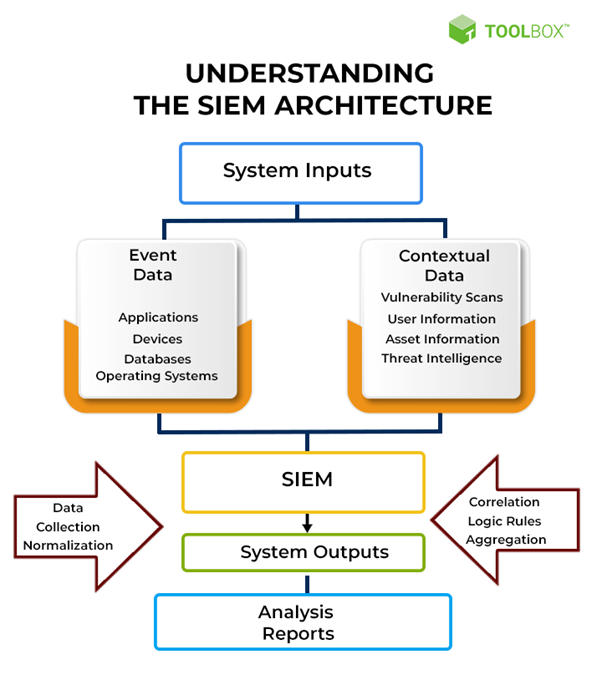
\includegraphics[width=0.55\textwidth]{assets/2_p1.png}
   \caption[Allgemeine Struktur von \gls{SIEM}]
   {Allgemeine Struktur eines \gls{SIEM}\\Quelle: \citep{Mohanan_What} }
   \label{fig:SIEM_Allg_Struktur}
   \centering
\end{figure}

Obem auf dem Bild, sehen wir, dass es zwei wichtige Datenquelle gibt, auf der linken Seite sind die Logdateien der \glsplural{Endpoint} und auf der rechten Seite die Informationen, um Anomalie zu erkennen. Nur der linken Seite stellt ein Log-Analyse-Tool dar. Mit der Nutzung der Elementen der rechten Seite, werden die Daten verarbeitet, um Muster zu erkennen und Information herauszuholen. Diese Zusammenarbeit repräsentiert eine \gls{SIEM}-Lösung, die als Ergebnis ein oder mehrere Berichten und/oder Graphik ausgeben kann. \cite{Granadillo_SIEM} teilt ein \gls{SIEM} in unabhängige Blöcke auf, wo jeder Block eine spezifische Funktion hat. Diese Blöcke und die Richtung der Information werden werden in der Abbildung \ref{fig:SIEM_Allg_Informationsfluss} dargestellt:


% \textbf{\textcolor{red}{Graphik selbst bauen}}

% \begin{figure}[H]
%    \centering
%    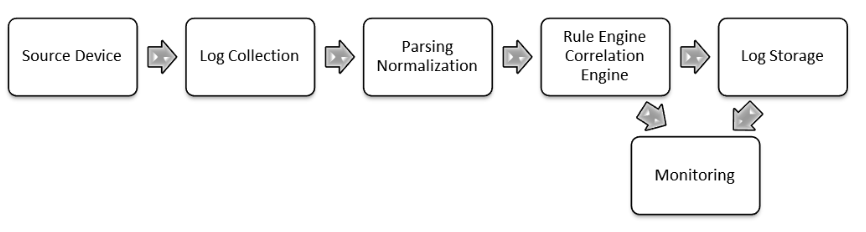
\includegraphics[width=0.8\textwidth]{assets/2_p2.png}
%    \caption[Allgemeine Informationsfluss von \gls{SIEM}]
%    {Allgemeine Informationsfluss eines laut \cite{Granadillo_SIEM} }
%    \label{fig:SIEM_Allg_Informationsfluss}
%    \centering
% \end{figure}

\begin{figure}[H]
   \centering
   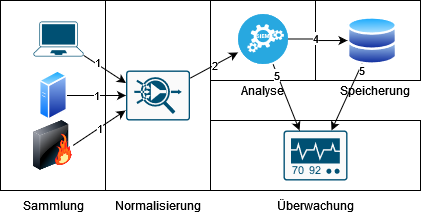
\includegraphics[width=0.8\textwidth]{assets/InfoFluss_SIEM.png}
   \caption[Allgemeine Informationsfluss von \gls{SIEM}]
   {Allgemeine Informationsfluss eines nach \cite{Granadillo_SIEM} }
   \label{fig:SIEM_Allg_Informationsfluss}
   \centering
\end{figure}



In der Abbildung \ref{fig:SIEM_Allg_Informationsfluss} sehen wir den Informationsfluss, wo die Logdateien erstellt werden, bis ihr Inhalt bearbeitet und verarbeitet wird. Die Logdateien der \glsplural{Endpoint} werden von einem sogenannten \textit{collector} gesammelt (1). Diese werden dann angepasst, damit sie eine einheitliche Formatierung bekommen (2), da sie verschiedene Format und Inhalte beinhalten. Danach werden die normalisierten Daten analysiert und nach Angriffsmuster verarbeitet (3). Der Inhalt wird dann in einer Datenbank gespeichert (4) und sowohl das Ergebnis der Analyse als auch der Inhalt können von einer Überwachungstool in Graphik- und/oder Textformat aufgerufen werden (5) \cite{Granadillo_SIEM}. 

% Die folgende Abbildung zeigt eine allgemeine Architektur von Log-Analyse-Tools:

% \begin{figure}[H]
%    \centering
%    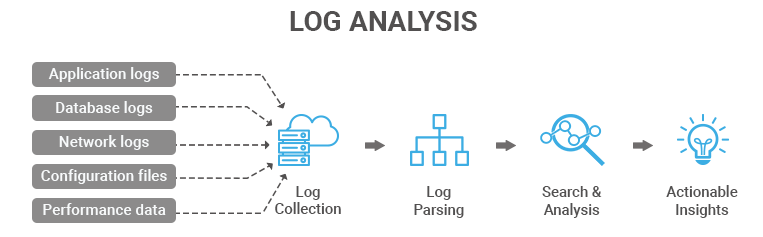
\includegraphics[width=0.8\textwidth]{assets/2.1_p2.png}
%    \caption[Allgemeine Struktur von Log-Analyse-Tools]
%    {Allgemeine Struktur von Log-Analyse-Tools\\Quelle: \citep{Tek-Tools_LGTArchitektur} }
%    \centering
% \end{figure}

% Den Informationsfluss eines Log Analyse Tools bildet folgende Grafik ab:

% \begin{figure}[H]
%    \centering
%    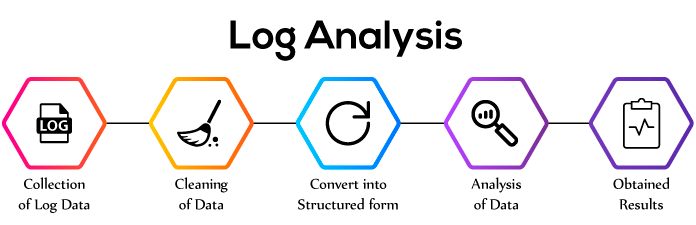
\includegraphics[width=0.55\textwidth]{assets/2.2_p2.png}
%    \caption[Allgemeine Informationsfluss von Log-Analyse-Tools]
%    {Allgemeine Informationsfluss von Log-Analyse-Tools\\Quelle: \citep{Neptune_LATInfoFluss} }
%    \centering
% \end{figure}

Aus bisheriger Abbildung stellen wir fest, dass \gls{SIEM} das Ergebnis der Integration von zwei wichtigen Komponenten ist, Datensammlung und Verarbeitung. Das Ziel dieser Software ist es die automatische Analyse zu ermöglichen, indem Daten kombiniert und bewertet werden können. In vielen Bereichen, wie Finanzen (\glsfirst{PCDISS}), Gesundheitswesen (\glsfirst{HIPAA}), sind \glsplural{SIEM} eine gesetzliche vorgegeben \citep{Jog_SIEM}. In Deutschland verpflichtet das \gls{IT-Sicherheitsgesetz 2.0} die Anwendungen solcher Lösungen, um Schädigung der \glsfirst{CIA} zu verhindern \citep{BSI_ITSG}. Log-Analyse-Tools sind seinerseits allgemeine Tools zu der Speicherung, Anpassung, Bewertung und Darstellung von Logdateien, ohne dass sie sich auf die Sicherheitsebenen fokussieren.

\subsection{Existierende SIEMs Lösungen und Log-Analyse-Tools}
Die existierenden \glsplural{SIEM} und Log-Analyse-Tools werden in \textit{\gls{Proprietary}} und \textit{\gls{opensource}} getrennt. In folgenden Abschnitten präsentieren wir das \textit{\gls{Proprietary}}e Tool Splunk, um einen Maßstab für unsere Auswahl über Funktionalität zu definieren. Wir analysieren folgende Tools: %\glsplural{SIEM} und Log-Analyse-Tools:

\begin{itemize}[noitemsep]
   \item Prelude %(nein)
   \item AlienVault \glsfirst{OSSIM} %(nein)
   \item FortiSIEM %(nein)
   \item Elastic Stack %(nein)
   \item Grafana integriert mit Loki %(ja)
\end{itemize}

\subsubsection{Splunk}
Splunk, von dem gleichnamigen Unternehmen, wurde 2003 in den USA auf dem Markt gebracht \citep{Splunk_splunk}. Splunk bietet einfache Wartung, benutzerfreundliche \gls{GUI} und Skalierbarkeit \citep{Kazarov_Splunk}. Er gehört zu der meistverwendeten \gls{SIEM} und zu ihren Kunden gehören große Konzerne wie Airbus, Coca-Cola, Intel und die Deutsche Bahn. Splunk bietet laut seiner Webseite folgende Funktionalitäten an \citep{Splunk_SPE}:

\begin{itemize}[noitemsep]
   \item Skalierbare Datenplattform
   \item Risk-based Warnmeldung
   \item Bedrohungserkennung mithilfe von \glsfirst{ML}
   \item Automatische Aktualisierung von der Bedrohungs- und Schwachstelle-Database
   \item Unkomplizierte Installation und Anwendung
\end{itemize}

Die Architektur und der Informationsfluss von Splunk unterscheidet sich nicht von der oben dargestellten Struktur in der Abbildung \ref{fig:SIEM_Allg_Struktur} und Abbildung \ref{fig:SIEM_Allg_Informationsfluss}. Da es sich hier um eine proprietäre Lösung handelt, lässt sich Splunk mit anderen Funktionalitäten verwalten und erweitern.

Die nächste Abbildung, \ref{fig:Allgemein_Splunk}, zeigt ein zusammenfassendes Diagramm über den Umfang des Informationsflusses von Splunk laut \cite{Splunk_platform}:

% % \begin{figure}[H]
% %    \centering
% %    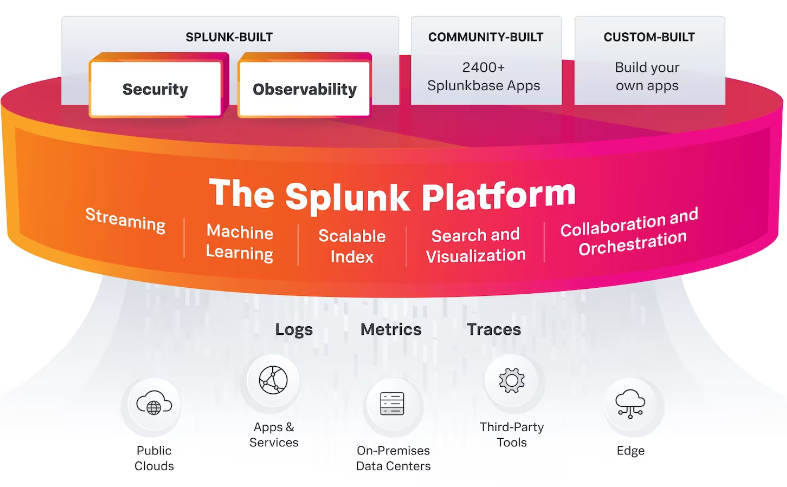
\includegraphics[width=0.7\textwidth]{assets/Splunk_informationsfluss.png}
% %    \caption[Allgemeine Informationsfluss von Splunk]
% %    {Allgemeine Informationsfluss von Splunk\\Quelle: \citep{Splunk_platform} }
% %    \label{fig:Allgemein_Splunk}
% %    \centering
% % \end{figure}

\begin{figure}[H]
   \centering
   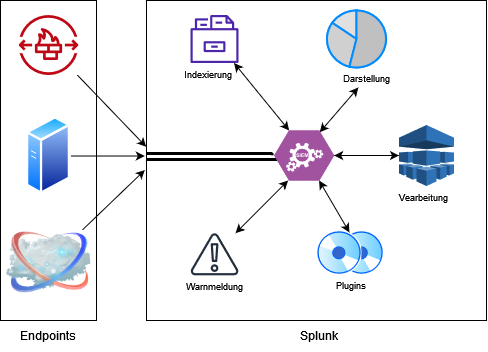
\includegraphics[width=0.5\textwidth]{assets/Splunk.drawio.png}
   \caption[Allgemeine Informationsfluss von Splunk]
   {Allgemeine Informationsfluss von Splunk}
   \label{fig:Allgemein_Splunk}
   \centering
\end{figure}

%Auf der Abbildung \ref{fig:Allgemein_Splunk} haben wir unten die \glsplural{Endpoint}, dessen Logdateien von Splunk und seine \glsplural{plugin} und Funktionalitäten verarbeitet und analysiert werden.

Auf der Abbildung \ref{fig:Allgemein_Splunk} haben wir links die \glsplural{Endpoint}, dessen Logdateien von Splunk und seine \glsplural{plugin} und Funktionalitäten (rechts) verarbeitet und analysiert werden. Der Konzept von Splunk lässt sich von der Idee formulieren, dass verschiedenen und unabhängige Funktalitäten zusammenarbeiten \citep{Splunk_platform}.

\newpage
Wie in anderen Tools, funktioniert die Bedrohungserkennung mithilfe von Regelsätzen, die aus \glsplural{usecases} entstehen. Laut der Dokumentation existieren sie in folgenden Szenarien: Überwachung, Untersuchung und Erkennung. Die Software ist sowohl mit \gls{mitre} Matrix als auch mit \glsfirst{CKC} für die Gestaltung ihrer \glsplural{usecases} integriert \citep{Splunk_usecases}.

In \citep{Su_SplunkDDOS} wurden Angriffe auf einem System simuliert und schließlich mit Splunk analysiert, um Gefahren zu identifizieren und diese im Voraus zu sehen. In \citep{Selvaganesh_SplunkBruteForce} wurde beschrieben, wie eine Splunk-Instanz installiert und konfiguriert wird, um spezifische \gls{bruteforce} zu erkennen.

\subsubsection{Prelude}
% suche nach Modulen, die man separat benutzen kann (Correlator)
Das im Jahr 2002 in Frankreich von Yoann Vandoorselaere released Tool Prelude zählt zu einer europäischen \gls{opensource} \gls{SIEM} Lösung. Laut dem Anbieter verfügt Prelude unter anderem folgende Funktionalitäten \citep{Prelude_SIEM}:

\begin{itemize}[noitemsep]
   \item	Informationszentralisierung
   \item	Datenaggregation und -Zusammenhang mit vordefinierten und von dem Nutzer angepassten Regeln
   \item	Einbruchserkennungsmechanismen
   \item	Datennormalisierung
\end{itemize}

Die Anwendung besteht aus verschiedenen unabhängigen Modulen. Unter denen nennen wir Warnmeldung, Archivierung, Analyse und Verwaltung. Erstens gehört zu der zentralen Aufgabe dieser Lösung - es kan folgendens: Daten empfangen, normalisieren, Zusammenhänge erschließen und Meldungen generieren. Das zweite Modul \quotes{Archivierung} konzentriert sich auf die Speicherung und Verfügbarkeit der Daten. Der Analyse-Modul stett Daten in verschiedenen Formaten dar. Das letzte Modul dient dazu, die Anwendung zu steuern, Nutzer zu erstellen und deren Rechte zu konfigurieren \citep{EC_Prelude}.

Die Abbildung \ref{fig:Module_preludes} zeigt die Integration verschiedener Module von Prelude und wie sie mit einander kommunizieren, um Analyse, Meldung und Speicherung zu generieren \citep{Prelude_MU}:

\begin{figure}[H]
   \centering
   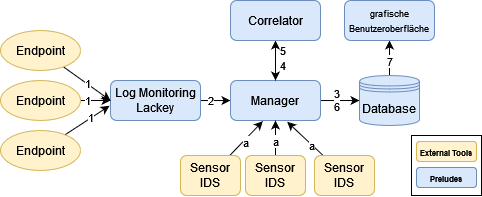
\includegraphics[width=0.8\textwidth]{assets/Prelude_Module.drawio.png}
   \caption[Integration zwischen den Modulen von Prelude ]
   {Integration zwischen den Modulen von Prelude }
   \label{fig:Module_preludes}
   \centering
\end{figure}

% \begin{figure}[H]
%    \centering
%    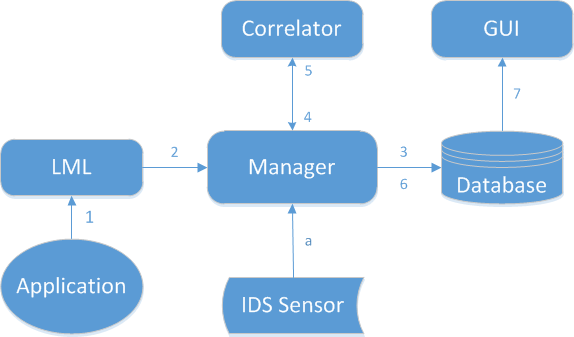
\includegraphics[width=0.5\textwidth]{assets/2_p3.png}
%    \caption[Integration zwischen den Modulen von Prelude ]
%    {Integration zwischen den Modulen von Prelude \\Quelle: \citep{Prelude_MU} }
%    \label{fig:Module_preludes}
%    \centering
% \end{figure}

Aus der Abbildung und der Dokumentation können wir folgenden Informationsfluss erkennen - die Daten werden von Endanwendung generiert und zum Loganalyzer (Prelude \glsfirst{LML}) (1) geschickt, wo sie normalisiert und bewertet werden Für die Logs, wo es verdächtige Werte nach dem vordefinierten Regelsätze in \gls{LML} gibt, werden Warnmeldungen generiert. Diese Meldungen werden zum Manager Module (2) weitergeleitet. Der Manager kann auch Daten von \gls{IDS} mithilfe von Sensoren empfangen (a), die an den \glsplural{Endpoint} installiert sind, um Events zu analysieren und zum Manager zu schicken. Die Daten werden in der Database gespeichert (3) und auch zu werden auch zum Correlator weitergeleitet, wo dieser nach einem Zusammenhang (5) zwischen anderen Daten sucht. Das Ergebnis von Correlator wird wieder zum Manager (4) geschickt und danach zu der Datenbank (6). Schließlich stehen die Berichte in dem \gls{GUI} (7) zur Verfügung \citep{Prelude_Doc}.

Die Architektur der Anwendung ermöglicht sowohl einen zentralisierten als auch einen dezentralisierten Aufbau, wie auf der Abbildung \ref{fig:Prelude_erweitert} gezeigt wird. In der ersten funktioniert Prelude als zentral und empfängt Daten von verschiedenen Datenquelle und in den zweiten gibt es mehrere sogenannten \quotes{Branches} von Preludes, dessen Ergenisse sich in einem \gls{GUI} darstellen lassen \citep{Prelude_MU}.

\begin{figure}[H]
   \centering
   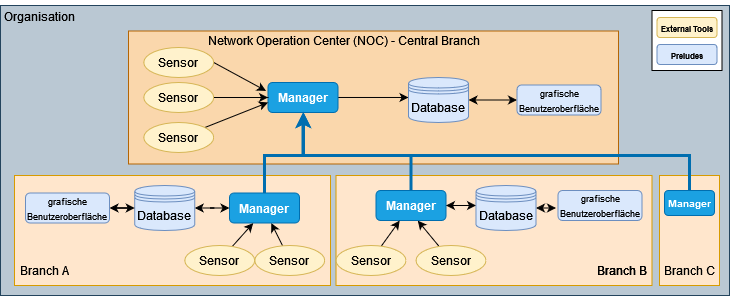
\includegraphics[width=1\textwidth]{assets/Branch_Prelude.drawio.png}
   \caption[Erweiterte Architektur von Prelude mit dezentralisierten Datenquellen und Datenverarbeitung]
   {Erweiterte Architektur von Prelude mit dezentralisierten Datenquellen Datenverarbeitung}
   \label{fig:Prelude_erweitert}
   \centering
\end{figure}

% % \begin{figure}[H]
% %    \centering
% %    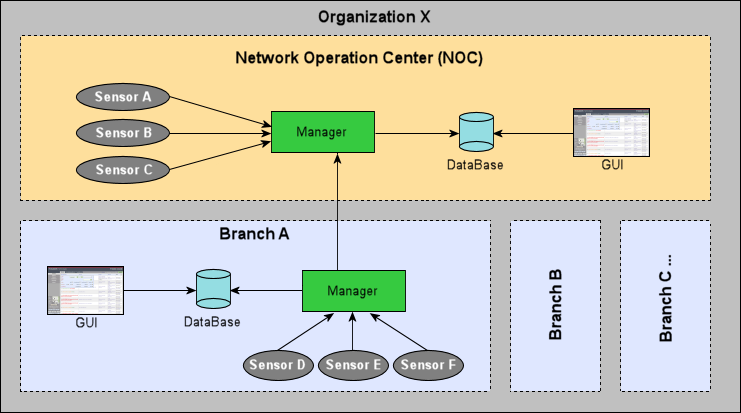
\includegraphics[width=0.8\textwidth]{assets/2_p5.png}
% %    \caption[Erweiterte Architektur von Prelude mit dezentralisierten Datenquellen und Datenverarbeitung]
% %    {Erweiterte Architektur von Prelude mit dezentralisierten Datenquellen Datenverarbeitung\\Quelle: \citep{Prelude_MU}}
% %    \label{fig:Prelude_erweitert}
% %    \centering
% % \end{figure}


%Die Darstellung einer dezentralisierte Umgebung von Preludes lässt sich in der folgenden Abbildung, \ref{fig:Prelude_erweitert}, darstellen:

% In der nächsten Abbildung, \ref{fig:Prelude}, sehen wir eine einfache Darstellung des Informationsflusses von Prelude:


In \citep{Grammatikis_Prelude} wurde Preludes, AlienVault und Cyberoam iView anhand technischer und nutzerfreundlicher Kriterien zu verglichen. Von diesn Kriterien nennen wir folgende \citep{Grammatikis_Prelude}:

\begin{itemize}[noitemsep]
   \item \textbf{technische Kriterien}
   \begin{itemize}[noitemsep]
      \item Echtzeige Leistung %\textit{Real-time performance},
      \item Umfang und Flexibilität der Meldungen %\textit{Range and flexibility of reporting}
      \item Zusammenhang von Warnmeldung %\textit{Alert correlation}
   \end{itemize}

   \item \textbf{nutzerfreundliche Kriterien}
   \begin{itemize}[noitemsep]
      \item Vollständige Dokumentation %\textit{Documentation comprehensiveness}
      \item Schwierigkeitsgrad der Installation %\textit{Complexity of the installation process}
      \item Schwierigkeitsgrad der Einstellung %\textit{Complexity of the system configuration}
   \end{itemize}
\end{itemize}

In den technischen Kriterien lag Prelude auf dem dritten Platz und bei Benutzerfreundlichkeit bekam Prelude den ersten.

\subsubsection{AlienVault OSSIM}
AlienVault OSSIM ist eine im Jahr 2007 entwickelte \gls{opensource} \gls{SIEM} Lösung. Im Jahr 2018 wurden sie von der Firma AT\&T Communication gekauft  \citep{CBN_AV}. In der Beschreibung des Anbieters steht, dass er sie auch dabei unterstützt, Daten zu sammeln, zu normalisieren und zu bewerten. Er behauptet auch, dass sein Tool in der Lage ist, Schwachstellen und Angriffe zu erkennen, das Verhältnis zu beobachten und Datenzusammenhänge zu erschließen \citep{ATT_AVO}.

AlienVault hat eine kostenpflichtige Version, die Alien Vault \glsfirst{USM} heißt. Auf der Webseite von AT\&T steht, dass es keine dedizierte Dokumentation für die \gls{opensource} Version AlienVault OSSIM gibt, da viele Funktionalitäten von der kostenpflichtigen Version stammen \citep{ATT_AVO}.

Die nächste Abbildung \ref{fig:AlienVault_Architektur} stellt das von dem Anbieter freigelegte Architekturdiagramm von der \gls{USM} Version dar \citep{ATT_AVO}:

\begin{figure}[H]
   \centering
   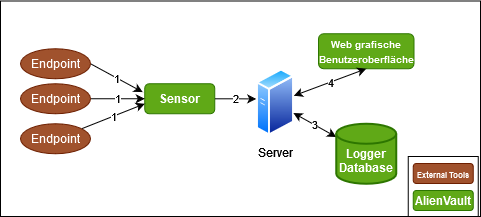
\includegraphics[width=0.7\textwidth]{assets/AlienVault.drawio.png}
   \caption[Architekturdiagramm von AlienVault \gls{USM}]
   {Architekturdiagramm von AlienVault \gls{USM}}
   \label{fig:AlienVault_Architektur}
   \centering
\end{figure}


% \begin{figure}[H]
%    \centering
%    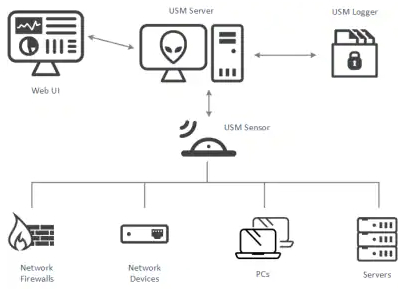
\includegraphics[width=0.6\textwidth]{assets/2_p6.png}
%    \caption[Architekturdiagramm von AlienVault \gls{USM}]
%    {Architekturdiagramm von AlienVault \gls{USM} \\Quelle: \citep{ATT_AVO} }
%    \label{fig:AlienVault_Architektur}
%    \centering
% \end{figure}

Links auf der Abbildung \ref{fig:AlienVault_Architektur} sehen wir die mit einem Sensor verbundenen \glsplural{Endpoint} (1). Der Sensor analysiert die Daten und leitet diese zu dem Server (2) weiter \citep{AV_Sensor}. Die Daten werden auf Logger (3) gespeichert und über die \gls{GUI} (4) dargestellt.

Laut der Website Comparitech steht AlienVault auf dem 13ten Platz von den bestbewertetsten \gls{SIEM}-Lösungen. Die Seite beschreibt auch, dass zu dem Tool einen \gls{IDS}, ein Verhaltensüberwachungssystem und einen Schwachstellen-Scanner integriert sind. Die Anwendung ist auch mit der Plattform \gls{OTX} verbunden - diese ermöglicht eine Teilung von Informationen über die Schwachstelle. Comparitech highlighted, dass die Anwendung wegen ihrer niedrigen Kosten besser für kleine oder mittelständige Unternehmen geeignet ist \citep{comparitech_SIEM}.

Die Anwendung bietet konsistenten Daten Zusammenhang an und soll das Auftauchen von \gls{falsch positiv} vermeiden. AlienVault kommt mit vordefinierten \glsplural{usecases}, die dabei unterstützen, gewöhnliche Angriffsszenarien zu erkennen. Die Installation, die Einstellung und die Integration mit anderen Tools ist auch benutzerfreundlich \citep{Gomes_AV}. \citep{Nabil_AV} behauptet, dass für viele Quellen eine manuelle Normalisierung der Logdatein notwendig ist.

%Die Anwendung hat aber einen zuverlässigen Berichtsmechanismus.

%Während unserer Recherche gab es wenig wissenschaftliche Literatur, die sich um AlienVault OSSIM kümmert.
Die meisten Publikationen über AlienVault OSSIM stammen aus kommerziellen Quellen und diese konzentrierten sich auf eine kostenpflichtige \gls{SIEM}-Lösung von AT\&T.

\newpage
\subsubsection{FortiSIEM}
FortiSIEM ist eine \gls{SIEM}-Lösung von der US-amerikanische Firma Fortinet. Fortinet kaufte im Jahr 2016 das Unternehmen AccelOps und dessen \gls{SIEM}-Lösung und benannte es zum FortSIEM \citep{Fortinet_Press}.

Laut dem Anbieter hat FortiSIEM eine robuste Integration mit anderen Tools und lässt sich leicht und einwandfrei skalieren. Andere Versionen des Tools sind mit \glsfirst{ML} integriert, sodass die Anwendung auch Verhältnisanalysen durchführen kann \citep{Fortinet_Solutions}. Das Tool bietet auch eine umfangreiche und ausführliche Dokumentation an. Die nächste Abbildung, \ref{fig:FortiSIEM}, zeigt die skalierbare Architektur von FortiSIEM:

\begin{figure}[H]
   \centering
   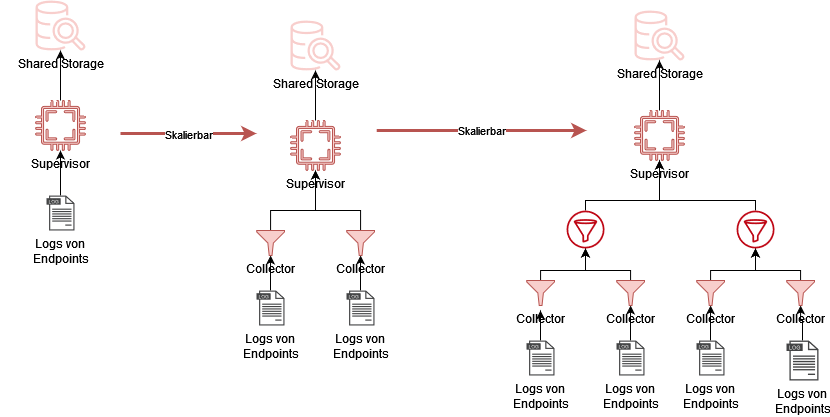
\includegraphics[width=1\textwidth]{assets/FortSIEM.drawio.png}
   \caption[Skalierbare Architektur von FortiSIEM]
   {Skalierbare Architektur von FortiSIEM laut \cite{Fortinet_Arch} }
   \label{fig:FortiSIEM}
   \centering
\end{figure}

Auf der linken Seite der Abbildung \ref{fig:FortiSIEM} haben wir eine einfache Struktur, wo die Logdatei zu dem \quotes{Supervisor} geschickt ist. Diese ist für die Analyse und Darstellung der Daten zuständig. Wenn die Architektur skaliert (mitte), kommen die \quotes{Collectors}. Diese tragen dazu bei, die Skalierbarkeit zu unterstützen, da sie Logdateien aus verschiedenen Quellen empfangen und normalisieren.Auf weitere Erweiterung kommen dann die \quotes{Workers}, die die Datananaylse durchführen und für die Database zuständig ist \citep{Fortinet_Key}.

% \textbf{\textcolor{red}{Graphik selbst bauen}}
% \begin{figure}[H]
%    \centering
%    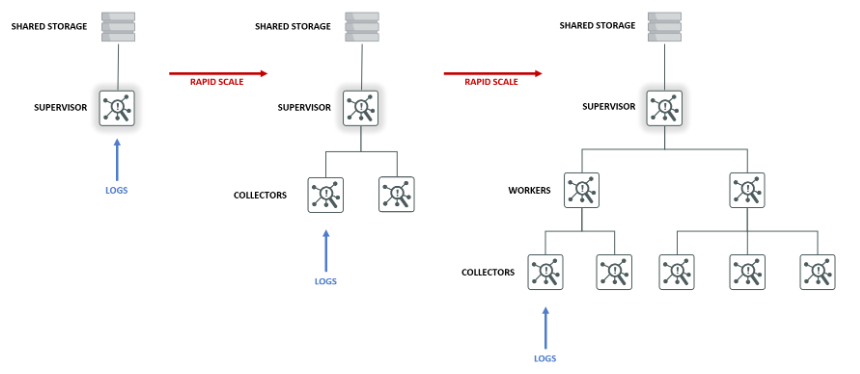
\includegraphics[width=1\textwidth]{assets/2_p7.png}
%    \caption[Skalierbare Architektur von FortiSIEM]
%    {Skalierbare Architektur von FortiSIEM \\Quelle: \citep{Fortinet_Arch} }
%    \label{fig:FortiSIEM}
%    \centering
% \end{figure}

\citep{Ramires_fortsiem} behauptet, dass FortiSIEM eine schnelle Erkennung von Angriffen bietet und über \glsfirst{NOC} Funktionalität verfügt, wie Netzmanagement.Wie andere \glspl{SIEM} Lösungen, biete FortiSIEM die folgenden Funktionalitäten: Datensammlung und Normalisierung, Daten Zusammenhang, Generierung von Berichten, Warnmeldungen, Datenauswertung.

% \begin{itemize}[noitemsep]
%    \item Datensammlung und Normalisierung
%    \item Daten Zusammenhang
%    \item Generierung von Berichten
%    \item Warnmeldungen
%    \item Datenauswertung
% \end{itemize}

\subsubsection{Elastic Stack}
Elastic Stack stammt aus der Verbindung von drei Tools: Elasticsearch, Logstash und Kibana. Erstes ist eine Such-und Analyse-Maschine. Das Zweite ist eine serverseitige Anwendung zur Datenverarbeitung, -Weiterleitung und Sammlung von Logdateien. Schließlich Kibana \label{kibana} ist eine \gls{abfragesprache} dafür zuständig, Daten zu filtern und visuelle Darstellungen in einem Grafik-Format auszugeben \citep{packt_elkstack}. Von diesen drei Tools Logstash ist das einzige \gls{opensource} \citep{elastic_OSI}. Obwohl die anderen zwei
kostenlos verwendet werden können, gehören sie nicht zu der \gls{opensource} Kategorie \citep{OpenSource_Def}. Dieses Tool besitzt viele Eigenschaften einer \gls{SIEM}-Lösung und wird von vielen SOC verwendet, ist aber für viele Experten, kein \gls{SIEM} für sich, da es über keine Warnmeldungssystem, Daten Zusammenhang und Vorfälleverwaltung verfügt \citep{Miller_ELK}. Diese und anderen Funktionalitäten lassen sich aber durch \glsplural{plugin} integrieren.

Die nächste Abbildung, \ref{fig:Intregation_ELK}, stellt die Architektur von Elastic Stack mit ihren integrierten Elementen dar:

\begin{figure}[H]
   \centering
   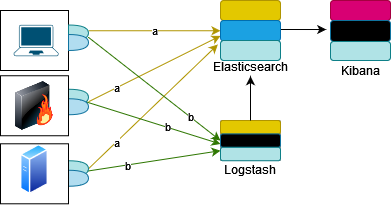
\includegraphics[width=0.6\textwidth]{assets/ElasticStack.png}
   \caption[Integration zwischen Elasticsearch, Logstash und Kibana]
   {Integration zwischen Elasticsearch, Logstash und Kibana laut \cite{packt_elkstack} }
   \label{fig:Intregation_ELK}
   \centering
\end{figure}

% \textbf{\textcolor{red}{Graphik selbst bauen}}

% \begin{figure}[H]
%    \centering
%    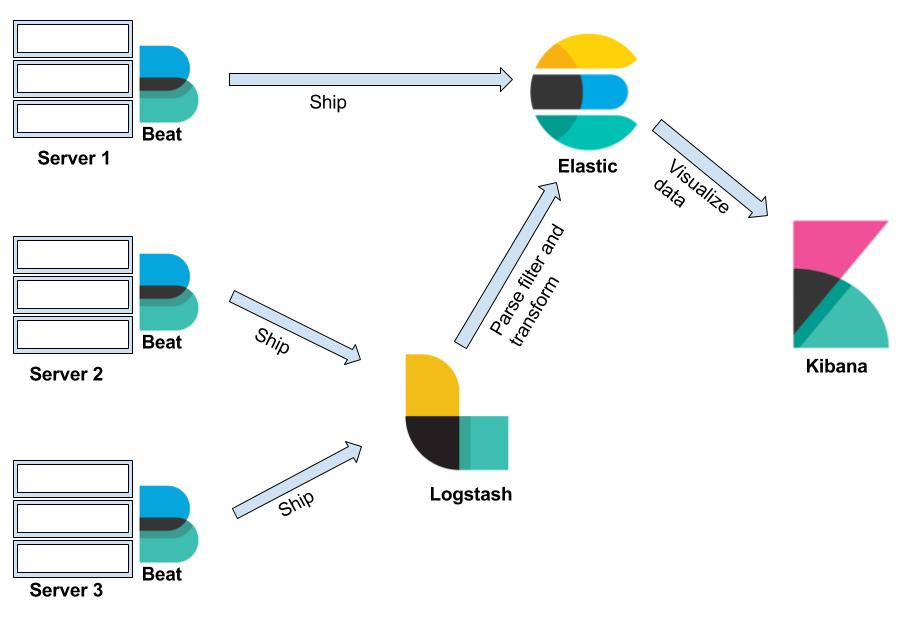
\includegraphics[width=0.8\textwidth]{assets/2_p8.png}
%    \caption[Integration zwischen Elasticsearch, Logstash und Kibana]
%    {Integration zwischen Elasticsearch, Logstash und Kibana\\Quelle: \citep{packt_elkstack} }
%    \label{fig:Intregation_ELK}
%    \centering
% \end{figure}

% \glsplural{Endpoint}
%\gls{abfragesprache} \gls{DSL}

Die Beats auf der Abbildung sind an der \glsplural{Endpoint} installiert und leiten Daten entweder zu Elasticsearch (a) oder zu Logstash (b) weiter. In Elasticsearch werden die Daten nach Muster mithilfe der Abfragesprache \glsfirstplural{DSL} gesucht. In Logstash werden die Daten verarbeitet, gespeichert und weitergeleitet. Schließlich ist Kibana für die graphische Darstellung über die \gls{GUI} zuständig \citep{Jain_LMELK}.

%Die Beats auf der Bild sind an der \glsplural{Endpoint} installiert und leiten Daten entweder zu Elasticsearch oder zu Logstash weiter, wo sie schließlich bearbeitet werden \citep{Jain_LMELK}.

In \citep{Advani_elkstakc} wird über die Log Analyse-Funktionalitäten von Elastic Stack und die Unterstützung bei Normalisierung und Indexierung von Daten für eine lesbare Ausgabe recherchiert. Die Skalierbarkeit wurde in der Studie von \citep{Wang_elkwifi} erwähnt, wo Elastic Stack für Wi-Fi Logging eingesetzt wurde.

Die offizielle Dokumentation von Elastic Stack beschreibt, dass die Anwendung folgende Funktionalitäten besitzt \citep{elastic_docs}:

\begin{itemize}[noitemsep]
   \item Datensuche, -Normalisierung, -Analyse und
   \item Speicherung
   \item visuelle Ausgabe
\end{itemize}

Die nächste Abbildung, \ref{fig:ElasticKomponenten} zeigt laut der offiziellen Dokumentation die Aufteilung der Funktionalitäten pro Element von Elastic Stack:

\begin{figure}[H]
   \centering
   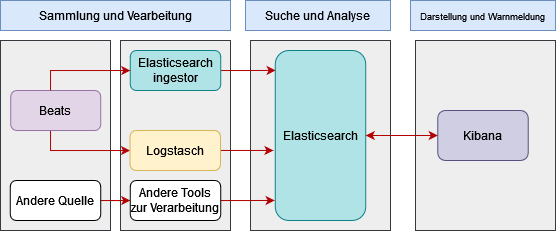
\includegraphics[width=0.8\textwidth]{assets/ELK_Architektur.png}
   \caption[Aufteilung der Funktionalitäten zwischen den Komponenten]
   {Aufteilung der Funktionalitäten zwischen den Komponenten}
   \label{fig:ElasticKomponenten}
   \centering
\end{figure}

Die aufgeteilte Struktur auf der Abbildung \ref{fig:ElasticKomponenten} hat die folgende Komponenten: die \quotes{Ingestor} für das Hinzufügen, die Sammlug und die Anpassung des Inhalts der Logdateien; die Speicherung, wo die Daten analysiert werden und schließlich der \quotes{Verbrauchen}, wo die Darstellung und die Warnmeldungen stattfinden \citep{elastic_docs}.

% \begin{figure}[H]
%    \centering
%    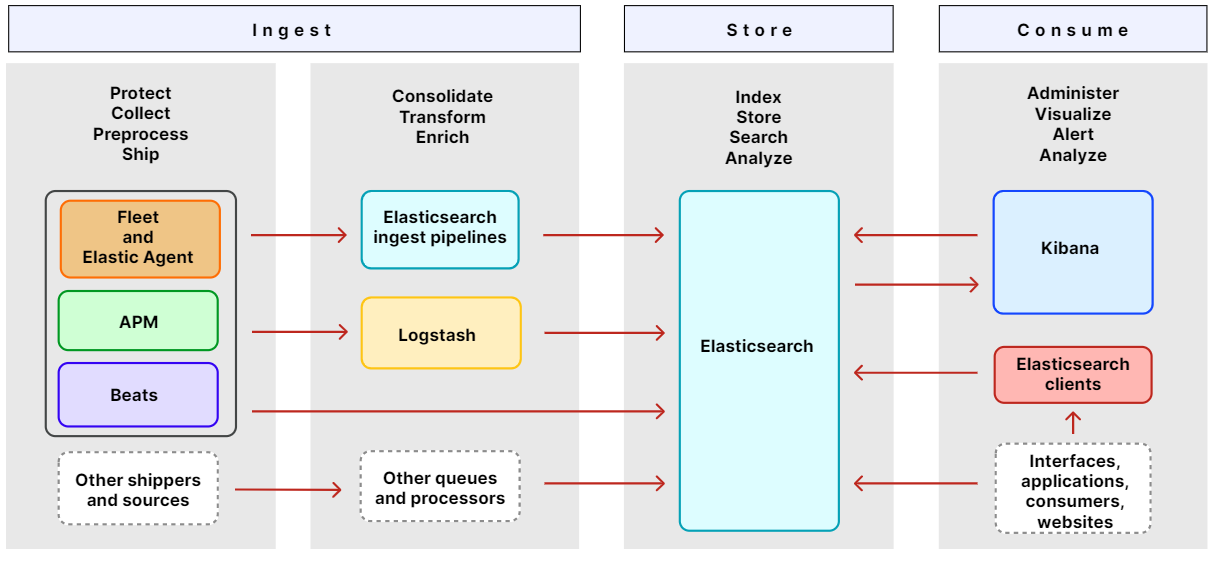
\includegraphics[width=0.8\textwidth]{assets/2_p9.png}
%    \caption[Aufteilung der Funktionalitäten zwischen den Komponenten]
%    {Aufteilung der Funktionalitäten zwischen den Komponenten\\Quelle: \citep{elastic_docs}}
%    \label{fig:ElasticKomponenten}
%    \centering
% \end{figure}

Die wissenschaftliche Publikation über Elastic Stack ist vielfältiger als bei anderen recherchierten Tools. Die Mehrheit von denen sich eher mit dem Logging als mit den \gls{SIEM}-Eigenschaften der Anwendung beschäftigt.

\subsubsection{Grafana}
Von allen recherchierten Lösungen ist Grafana die Einzige, die weder \gls{SIEM} noch Log-Analyse-Tools ist. Grafana wird als Plattform für Visualisierung von Daten beschrieben. Mit dem Tool ist es möglich eine Graphik zu erstellen und Meldungen zu generieren. Das Ziel der Anwendung ist, Information in einer einfachen und verständlichen Art und Weise zur Verfügung zu stellen \citep{redhat_grafana}.

Im Jahr 2014 wurde Grafana von der Firma Grafana Labs veröffentlicht. Ursprünglich sollte Grafana ein einfacheres Bearbeitungstool für Grafiken sein und ermöglichen, Datenanfragen unkomplizierter zu machen. Es ist auch möglich das Grafana mithilfe von \glsplural{plugin} zu erweitern \citep{Oedegaard_historyGrafana}.

In der Webseite betont der Anbieter, dass Grafana die Zentralisierung und Zugang von Daten vereinfachen. Alle Art von Daten lassen sich analysieren und darstellen, von der Leistung von Anwendungen bis Verkaufsdaten und Krankheitsfällen. Die Anwendung soll auch den Zusammenhang von Daten ermöglichen, um wichtige Informationen herauszunehmen \citep{Grafana_Grafana}. Grafana ermöglicht die Aufrufe der Daten mithilfe von verschiedenen \gls{abfragesprache}, jenachdem mit welchen Datenquelle verwendet wird. Das Tool bietet auch eine eigene Funktionalität, um Warnmeldung zu generieren oder lässt sich mit externen Tools, wie Alertmanager von \gls{prometheus}, integrieren. 

Grafana ist auch mit dem Logging Tool Loki und Promptail integriert. Promtail ist für Sammlungen der Logdateien und Weiterleitung an Loki zuständig während Loki sich um die Speicherung, Indexierung und Abfrage kümmert.

Die Architektur von Loki besteht aus bla bla bla bla bla bla bla bla bla bla bla bla bla bla bla bla bla bla bla bla bla bla bla bla bla bla bla bla bla bla bla bla bla bla bla bla bla bla bla bla bla bla bla bla bla bla bla bla bla bla bla bla bla bla bilder. \gls{logql} 

%https://grafana.com/blog/2018/12/12/loki-prometheus-inspired-open-source-logging-for-cloud-natives/

bla bla bla bla bla bla bla bla bla bla bla bla bla bla bla 
bla bla bla bla bla bla bla bla bla Ingester, Distributor and Querier


Promptail wird an jeden \gls{Endpoint} installiert und er schickt als Stream zu Loki. Diese Streams werden dann in Loki mit Labels (Schlüssel-Wert-Paar) identifiziert. Jeder Stream bezieht sich auf eine Gruppe von Logdateien. Laut \cite{Grafana_fundamentals} bleibt der Inhalt der Logdateien ohne Indexierung, um Effizienz bei der Verwaltung des Inhalts zu gewinnen, im Vergleich zu anderen Tools, wie Elastic Stack, wo der gesammte Inhalt indexiert wird \citep{Anand_LokixELK}. Bei Loki werden die Metadata, wie Zeitstempel oder andere kundenspezifische Labels, dann indexiert.

Für eine optimale Nutzung wird von Grafana empfohlen, wenig \quotes{labels} zu benutzen, um eine Eskalation des Speicherbedarfs zu vermeiden \cite{Grafana_labels}. Die Abbildung \ref{fig:Eskalation_Labels} zeigt den Eskalationseffekt, der durch die Nutzung von \quotes{labels} entsteht:

\begin{figure}[H]
   \centering
   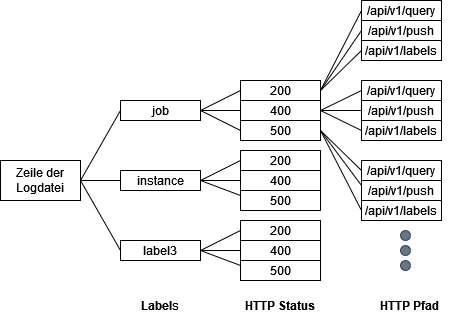
\includegraphics[width=0.7\textwidth]{assets/labelstream.png}
   \caption[Eskalation bei Verwendung von \quotes{labels}]
   {Eskalation bei Verwendung von \quotes{labels} laut \cite{Grafana_labels}}
   \label{fig:Eskalation_Labels}
   \centering
 \end{figure}
 
Auf Abbildung \ref{fig:Eskalation_Labels} haben wir vier Ebenen. Die erste ist die Zeile der Logdatei (1), die zweite sind die vom Benutzer definierten \quotes{labels} (2), und die dritte und vierte beziehen sich auf die Antwort (3) und die verwendete HTTP-Anfrage (4), um nach Inhalten zu suchen, sie hinzuzufügen und zu indizieren. Aus einer Zeile der Logdatei haben wir drei kundendefinierte \quotes{labels} definiert, die wiederum drei potenzielle Zustände haben. Aus diesen drei Zuständen haben wir drei mögliche \gls{http}-Pfade. Aus drei \quotes{labels} ergibt sich insgesamt 27 Streams, um die Zeile zu lesen, zu indizieren und zu speichern. Dies kann laut \cite{Grafana_labels} zu einer Beeinträchtigung der Leistung führen. Die folgende mathematische Formel zeigt das Ergebnis unserer Beschreibung:

{\setstretch{1.0}
\begin{Verbatim}[commandchars=\\\{\},frame=single]
Labels = 3
Anfrage = 3
HTTP-Antworte = 3
Total Streams = Labels x Anfrage x HTTP-Antworte
Total Streams = 3 x 3 x 3
Total Streams = 27
\end{Verbatim}
}

Promtail kann aber Logdateien nur zur Grafana Loki oder zu einem anderen Promtail Instanz schicken. In der Konfigurationsdatei von Promtail kann die Häufigkeit, in der nach neuem Inhalt in der Logdateien gesucht wird, konfiguriert werden. Auf Abbildung \ref{fig:Integration_Loki_Promtail_Grafana} wird die Verbindung zwischen Promtail und Grafana Loki dargestellt \citep{Grafana_Logs}:

% \begin{figure}[H]
%    \centering
%    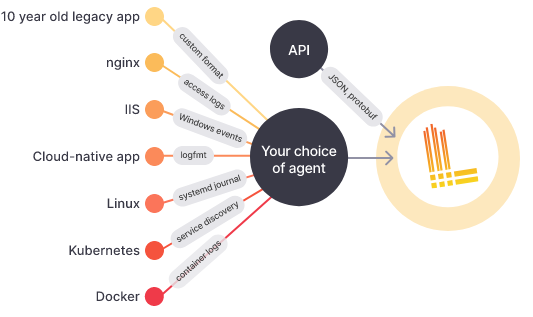
\includegraphics[width=0.8\textwidth]{assets/2_p10.png}
%    \caption[Integration von Log-Quellen mit Promptail, Loki und Grafana]
%    {Integration von Log-Quellen mit Promptail (links), Loki (mitte) und Grafana (rechts) \\Quelle: \citep{Grafana_Logs}}
%    \label{fig:Integration_Loki_Promtail_Grafana}
%    \centering
% \end{figure}

\begin{figure}[H]
   \centering
   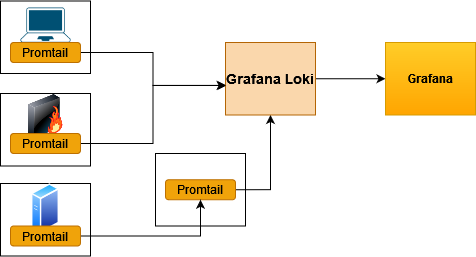
\includegraphics[width=0.8\textwidth]{assets/Promtail.png}
   \caption[Integration von Log-Quellen mit Promptail, Loki und Grafana]
   {Integration von Log-Quellen mit Promptail (links), Loki (mitte) und Grafana (rechts)}
   \label{fig:Integration_Loki_Promtail_Grafana}
   \centering
\end{figure}

. 

Die wissenschaftlichen Literatur über Grafana konzentriert sich eher auf die Anwendung des Tools für die grafische Darstellung von Daten als für ihre Nutzung in dem Sicherheitsbereich. Eine Recherche, z.B., wollte das Ergebnis von der Überwachung von Cloud-basierten Systemen, von Netzwerkaktivitäten und von Netzwerkverkehr mithilfe von Grafana darstellen \citep{Manases_grafananetwork}.
Die wissenschaftliche Recherche über die Implementierung und Integration von Grafana mit anderen Tools zum Sicherheitszweck ist neu und bietet deshalb viele  Perspektive für das Weiterlernen an.

\subsection{Auswahlkriterien}
Der Erwerb einer \gls{SIEM} Lösung würde wahrscheinlich die Anforderungen dieser wissenschaftlichen Arbeit decken. Da solche Lösungen meistens (oder alle) \gls{Proprietary} und kostenpflichtig sind, legten wir als Auswahlkriterium fest, dass die Anwendungen für unsere Arbeit \gls{opensource} sein müssen. Von allen analysierten Tools sind die Kombinationen Grafana, Loki, Promtail und Kibana, Elasticsearch, Logstash  am geeignetsten für unsere Auswahl. In der Tabelle \ref{tab:Vergleich_GrafanaELK} vergleichen wir beiden dieser Konbinationstool \citep{Anand_LokixELK}:

\begin{table}[H]
   \setstretch{1.2}
   \begin{tabularx}{\textwidth}{|c|c|X|}
   \hline
   \multicolumn{1}{|c|}{\textbf{Grafana}} & \multicolumn{1}{|c|}{\textbf{Elastic Stack}} & \multicolumn{1}{|c|}{\textbf{Gemeisame Rolle}} \\
   \hline
      Grafana & Kibana & \gls{frontend}, graphische Darstellung\\
   \hline
      Loki & Elasticsearch & \gls{backend}, Verarbeitung des Inhalts der Logdateien \\
   \hline
      Promtail & Logstash & \gls{backend}, Sammlung von Logdateien \\
      \hline
   \end{tabularx}
   \caption[Gemeinsamkeiten zwischen den Kombinationen Grafana, Loki, Promtail und Kibana, Elasticsearch, Logstash]
   {Gemeinsamkeiten zwischen den Kombinationen Grafana, Loki, Promtail und Kibana, Elasticsearch, Logstash}
   \label{tab:Vergleich_GrafanaELK}
\end{table}

Die nächste Tabelle, \ref{tab:Unterschiede}, fasst die Unterschieden zwischen den Tools zusammen:

{\setstretch{1}
\begin{table}[H]
   \centering
\begin{tabular}{|m{5cm}|m{4.2cm}|>{\centering\arraybackslash}m{4.2cm}|}
   \hline
   \centering\textbf{Eigenschaft} & \centering\textbf{Grafana, Loki und Promtail} & \textbf{Kibana, Elasticsearch und Logstash} \\ 
   \hline 
   Opensource                  & \centering
   ja & 
   nicht im Elasticsearch \\ \hline

   Dokumentation von Promtail und Logstash \citep{Kray_LogstashxPromtail} & \centering 
   einfach & Umfangreich \\ \hline
   
   Entwickelt spezifisch für Verarbeitung von Logdateien \citep{Yigal_GrafanaKibanan}  & \centering
   nein                    & 
   ja                      \\ \hline 

   Komplexität bei der Installation und Einstellung \citep{BetterStac_KG} & \centering 
   niedrig                &
   hoch                   \\ \hline 

   Komplexität bei der Installation und Einstellung \citep{BetterStac_KG} & \centering 
   niedrig                &
   hoch                   \\ \hline 

   Graphische Darstellung & \centering
   ja                     & 
   ja                     \\ \hline 

   Dashboards und Graphik  & \centering
   ja                      & 
   ja                      \\ \hline 

   Eigene \gls{abfragesprache} & \centering
   abhängig von dier Datenquelle (Grafana), \gls{logql} (Loki) & 
   \gls{DSL}               \\ \hline 

   Indexierung                & \centering
   nur Metadata (Loki)        &
    vollständog (Elasticsearch) \\ \hline 

   Dekomprimierung von Datei & \centering
   ja (Promtail)             &
   ja (Logstash)             \\ \hline 

   Integration mit anderen Database Tools & \centering
   ja                         & 
   nur mit Elasticsearch      \\ \hline

   Weiterleitung des Loginhalts & \centering
   nur an Promtail und an Loki (Promtail) &
   umfangreiche Integration mit anderen Tools (Logstash) \\ \hline

 \end{tabular}
 
\end{table}
}

{\setstretch{1}
\begin{table}[H]
   \centering
\begin{tabular}{|m{5cm}|m{4.2cm}|>{\centering\arraybackslash}m{4.2cm}|}
   \hline
   \centering\textbf{Eigenschaft} & \centering\textbf{Grafana, Loki und Promtail} & \textbf{Kibana, Elasticsearch und Logstash} \\ \hline 



   Integrietes Tool für Generierung von Warnmeldungen \citep{Yigal_GrafanaKibanan} & \centering
   ja (Alerting) & 
   von \glsplural{plugin} abhängig  \\ \hline

 \end{tabular}
 \caption{Unterschiede zwischen den Kombinationen Grafana, Loki, Promtail und Kibana, Elasticsearch, Logstash}
 \label{tab:Unterschiede}
\end{table}
}

Grafana erfüllt die folgende Voraussetzungen für unsere Auswahl: 100\% \gls{opensource}, einfacher Installation und Einstellung, integriertes Alerting Tool und breiter Kompatibilität (außer Promtail). Da Grafana nicht spezifisch für Logdateien konzipert wurde \citep{Yigal_GrafanaKibanan}, verlangt die Einstellung spezifische Anpassungen, um unseren Bedürfnisse vollständig zu erfüllen.

In den nächsten Kapiteln beschäftigen wir mit der Integration dieser Tools, um eine ähnliche \gls{SIEM} Lösung zu präsentieren. Wir beschreiben, wie Angriffe anhand der \glsfirst{ttp} der \gls{mitre} Matrix erkennt werden können. Wir simmulieren zwei Angriffe, um Logdateien zu generieren. Danach beschäftigen wir uns mit der Installation, Einstellungen und Sammlungen von Logdateien in Promtail, Grafana und Loki. Nachdem die Grundfunktionalitäten eingerichtet sind und einwandfrei funktionieren, untersuchen wir Regelsätze für die Erkennung und Warnmeldung von potenziellen Angriffe. Unser Ziel ist Grafana, Loki und Promtail so einzustellen, dass es in der Lage ist, die Muster dieser Angriffe zu erkennen und darüber zu berichten.